\chapter{How Are You Going to Make Money? The Business/Venture Model}

This lecture begins with a clean handoff. Bob Jones had already shown, in the preceding session, that customer choice and pricing choice are not afterthoughts; they are already the beginning of a business model. Rich Kivel now takes the next step in Joseph Hadzima's MIT OpenCourseWare course and asks the harder question: once we have an invention, a service, or a technology, how does it become revenue, investor return, and finally a sustainable business? The lecture answers this in a deliberate order. We are first given an operating story, then a definition, then a set of recognizable business-model types, then two major platform examples, and only after that a return to the industry-specific pressure of med tech. The notes should therefore unfold as the lecture unfolds: step by step, with each example motivating the next.

\section{From Customer Discovery to Business Model}

Kivel opens by making the scope of the evening unmistakable. We are no longer only asking who the customer is. We are asking how a company makes money, how it brings a product to market, and how it eventually produces returns for investors or strategic partners. In the lecture this is presented as the ``nitty-gritty'' of company building, and that phrase matters. The business model is not a slogan placed after the invention. It is the operating structure that carries the invention into economic life.

A compact reconstruction of the lecture's practical target is
\begin{equation}
\text{technology} \to \text{distribution} \to \text{adoption} \to \text{revenue} \to \text{sustainable business}.
\end{equation}
Kivel does not write this in symbols, but it is the underlying motion of the lecture. A technology by itself is inert from the standpoint of a company. Between invention and revenue there lie channels, buyers, behavior, and scale.

His autobiographical setup is also part of the argument. He presents himself as someone who spent the first part of his career on the operating side of companies: sales, marketing, partnerships, then CEO work, then investing. This is why the lecture does not begin with a framework diagram. It begins with operating experience. We are meant to see that a business model is discovered, stressed, and revised in contact with actual buyers.

\section{MolecularWare and the First Operating Model}

The first sustained example is the MIT spinout MolecularWare, a bioinformatics company from the era of the Human Genome Project. The technical scene is vividly drawn. A lab is full of autonomous devices: scanners, robots, micro-arrayers, barcode refrigerators, each with its own computer and its own software. The consequence is not elegance but spreadsheet chaos. Scientists and engineers become the unwilling clerks of disconnected systems.

Kivel's first important sequence comes here:
\begin{equation}
\text{capture} \to \text{visualize} \to \text{data mine} \to \text{create value}.
\end{equation}
This deserves to be preserved because it is the lecture's first clean reduction of a business problem to a usable structure. One first captures information from the instruments. One then visualizes it. Once the information is visible, one can interpret overexpression, underexpression, patterns, or anomalies. Only then does the downstream problem of data mining become meaningful, and only there does value begin to emerge in the commercial sense.

\begin{figure}[htbp]
\centering
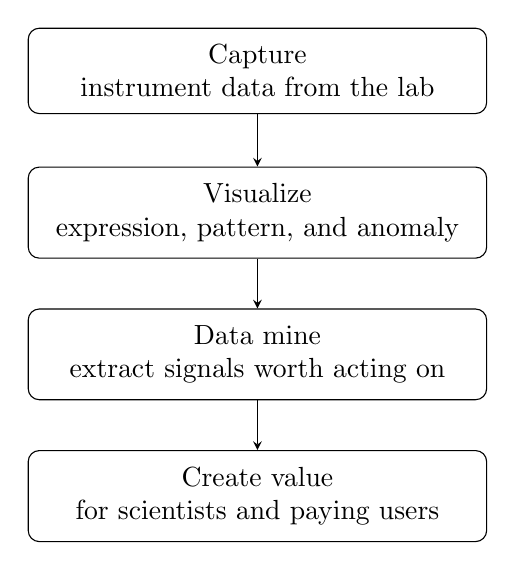
\begin{tikzpicture}[>=stealth]
\node[draw, rounded corners, align=center, text width=5.4cm, inner sep=6pt] (a) at (0,0) {Capture\\instrument data from the lab};
\node[draw, rounded corners, align=center, text width=5.4cm, inner sep=6pt] (b) at (0,-1.8) {Visualize\\expression, pattern, and anomaly};
\node[draw, rounded corners, align=center, text width=5.4cm, inner sep=6pt] (c) at (0,-3.6) {Data mine\\extract signals worth acting on};
\node[draw, rounded corners, align=center, text width=5.4cm, inner sep=6pt] (d) at (0,-5.4) {Create value\\for scientists and paying users};
\draw[->] (a) -- (b);
\draw[->] (b) -- (c);
\draw[->] (c) -- (d);
\end{tikzpicture}
\caption{Transcript-derived reconstruction of the MolecularWare value chain.}
\end{figure}

Kivel then makes a point that is easy to lose if we over-academicize the story. He had no background in biotech or pharma. He jokes that he did not know how even to spell bioinformatics. But the point is serious: what mattered was not disciplinary identity; what mattered was whether the company was creating value out of the invention. That is why he broadens the example from gene-expression labs to drones, satellites, emissions sensing, and other domains. The lecture's refrain is that the value often comes from the data.

From there he moves, with almost no pause, from product structure to channel structure. When he arrived as CEO, MolecularWare had one business model: it sold to academics. That made sense because the founders sold to the people they knew. It did not scale well, and it was not very attractive to the investment community. So the business model had to change:
\begin{equation}
\text{direct to academics} \to \text{distributors} \to \text{OEM}.
\end{equation}

The first extension was geographic. Building a sales force in Asia was impossible for a fifteen-person Kendall Square company, so distributors became the second part of the model. The second extension was even more decisive. The company had strong software and no reason to build instruments. Other firms had strong instruments and weak software. OEM bundling then becomes the elegant move: put the software inside the instrument and let the instrument company sell the complete system.

\begin{figure}[htbp]
\centering
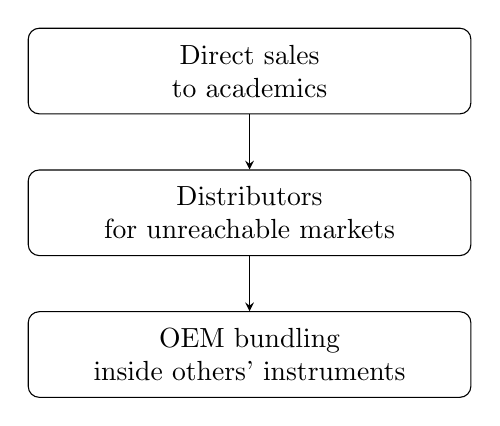
\begin{tikzpicture}[>=stealth]
\node[draw, rounded corners, align=center, text width=5.2cm, inner sep=6pt] (x) at (0,0) {Direct sales\\to academics};
\node[draw, rounded corners, align=center, text width=5.2cm, inner sep=6pt] (y) at (0,-1.8) {Distributors\\for unreachable markets};
\node[draw, rounded corners, align=center, text width=5.2cm, inner sep=6pt] (z) at (0,-3.6) {OEM bundling\\inside others' instruments};
\draw[->] (x) -- (y);
\draw[->] (y) -- (z);
\end{tikzpicture}
\caption{Transcript-derived reconstruction of the channel ladder in the MolecularWare case.}
\end{figure}

\subsection{Question \& Answer}

\paragraph{Question.} What is OEM, and why did it change the company?

\paragraph{Answer.} OEM means original equipment manufacturer. In the lecture it is not merely a vocabulary check. It is the moment at which the company changes how it reaches the buyer. MolecularWare stops trying to sell every installation itself and instead places its software inside another firm's instrument. The manufacturer now bears much of the burden of selling, distribution, and customer reach. MolecularWare receives value when the bundled instrument is sold. The route to market changes, and with it the economics of growth.

Kivel then generalizes from this example to his larger operating experience. He has taken companies
\begin{equation}
8 \to 85 \to 250 \to 1{,}000 \ \text{people},
\end{equation}
and he attributes that kind of growth not only to funding but to a business model flexible enough to support the growth. That claim prepares the ground for the formal definition.

\section{Definition, Flexibility, and the Nine-Part Canvas}

Only after the operating story does the lecture pause to define its subject. This order should be preserved. We are not given a framework and then asked to decorate it with examples. We are shown a company under pressure, and then we are given the abstraction that explains what we have just seen.

\begin{definition}
A business model describes the rationale by which an organization creates, delivers, and captures value.
\end{definition}

A faithful symbolic compression of the lecture's definitional core is
\begin{equation}
\text{Business model}=\text{create value}+\text{deliver value}+\text{capture value}.
\end{equation}

\begin{remark}
This displayed equation is a transcript-backed compression rather than a board-written formula. It is useful because it prevents us from treating creation, delivery, and capture as separable afterthoughts.
\end{remark}

Kivel then turns to the \emph{Business Model Generation} canvas and immediately refuses to let it become static. The nine components are not equal-sized slices of a permanent pie. Their weight changes with stage, financing, product maturity, and strategic pressure. They blend together. A manager may oversee key resources or key activities; a marketing team may be shaping the value proposition and the segmentation of customers; but the underlying claim is that these pieces must move together.

This is why the orchestra analogy appears. If the pieces of the model move harmoniously, the result is coherent. If one part lags or drifts, there are second- and third-order consequences. Cost structure is the lecturer's favored example. If the cost structure is not designed and revised properly, the firm starts to lose money; support weakens; repeat business fades; the model begins to damage itself.

There is a more general principle here, stated almost explicitly in the lecture: a successful business must be willing to modify its model quickly in response to the market. The model is not the frozen form of success. It is the mechanism by which a company remains able to move.

\section{A Menu of Canonical Models}

From the operating case and the formal definition, Kivel deliberately broadens the field. He reminds the room that none of this should feel exotic. We are all consumers. We live inside business models every day, whether or not we name them.

The lecture names a familiar cluster:
\begin{itemize}
\item subscription,
\item freemium,
\item marketplace,
\item advertising,
\item direct sales,
\item reseller,
\item OEM.
\end{itemize}

But the point is not taxonomy for its own sake. Kivel is training recognition. Years earlier, he says, business-model talk could feel almost arcane: are you going to sell online or retail, are you going to customize like Dell or stock inventory like everyone else? Then ubiquitous connectivity arrives, and suddenly models appear that would scarcely have made sense a short time before.

Subscription is introduced through ordinary life. We used to drive to Blockbuster, rent a movie, bring it home, and return it. There was no meaningful subscription in that world. The deeper shift, as Kivel phrases it, is from owning to experiencing. Freemium extends the same logic in another register: give access now, charge later, keep the user inside the system. Marketplace models let many sellers reach buyers through a shared platform. Advertising transforms attention into revenue rather than requiring equal direct payment from each user.

The older structures remain alive. Direct sales, reseller arrangements, and OEM still matter because the route to market is often the heart of the problem. In pharmaceutical biotech, direct sales forces survive because doctors are busy and physical education of the buyer still matters. The Intel example sharpens the point even further. Intel does not care very much about selling directly to end users. It sells to the manufacturer. In Kivel's improvised phrase, this is almost business-to-manufacturer.

The lecture therefore uses familiar models not to simplify the topic, but to show that the topic has been with us all along.

\section{Netflix as a Moving Target}

The lecture's first large platform example is Netflix. The narrative begins with Blockbuster, because Blockbuster makes the problem concrete. A retail chain owns stores, staffs them, secures them, manages inventory, handles returns, and charges late fees. Netflix appears first not as a studio or global streaming platform but as a company that mails DVDs.

That first move depends on the technological moment. Kivel stresses that at the beginning there was not enough bandwidth to make downloading a feature-length film practical. One could wait hours, consume memory, watch, delete, and repeat the process. The mailed-DVD model was not primitive. It was suited to the state of the world.

This first business model already contains several important features: convenience, no late fees, centralized inventory, and later a subscription layer that lets a household hold several DVDs out at once. The lecture is careful to keep the stages distinct. First there is mailing. Then there is the subscription tiering laid on top of mailing. Then the world changes.

Netflix does not survive by a theatrical leap of reinvention. It survives because it modifies its model before the old model becomes useless. Streaming enters gradually. Later, original content. Later, live events. Later still, small but powerful adjustments in pricing and account rules.

\subsection{Question \& Answer}

\paragraph{Question.} How did Netflix avoid dying with the DVD business?

\paragraph{Answer.} It did not mistake its first successful form for its permanent identity. Mailing DVDs solved the immediate distribution problem in a low-bandwidth world. Streaming solved the next problem. Original programming solved the problem of dependence on others' content. Live events open yet another line of relevance. The company survives not by discarding the old model in panic but by modifying it before the old logic is exhausted.

\begin{figure}[htbp]
\centering
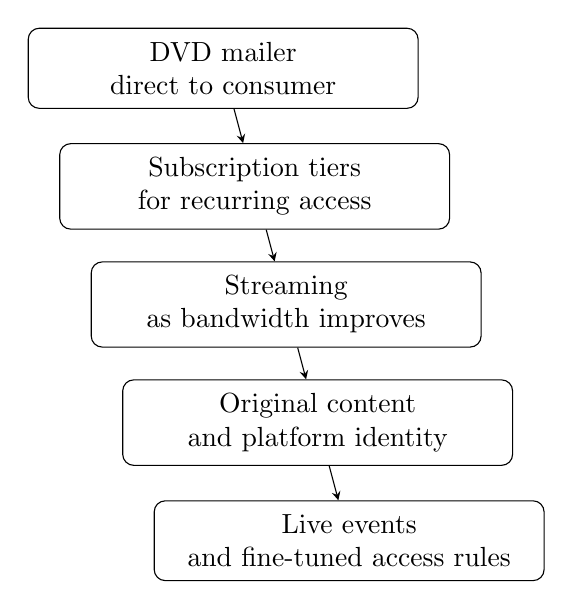
\begin{tikzpicture}[>=stealth]
\node[draw, rounded corners, align=center, text width=4.6cm, inner sep=5pt] (n1) at (0,0) {DVD mailer\\direct to consumer};
\node[draw, rounded corners, align=center, text width=4.6cm, inner sep=5pt] (n2) at (0.4,-1.5) {Subscription tiers\\for recurring access};
\node[draw, rounded corners, align=center, text width=4.6cm, inner sep=5pt] (n3) at (0.8,-3.0) {Streaming\\as bandwidth improves};
\node[draw, rounded corners, align=center, text width=4.6cm, inner sep=5pt] (n4) at (1.2,-4.5) {Original content\\and platform identity};
\node[draw, rounded corners, align=center, text width=4.6cm, inner sep=5pt] (n5) at (1.6,-6.0) {Live events\\and fine-tuned access rules};
\draw[->] (n1) -- (n2);
\draw[->] (n2) -- (n3);
\draw[->] (n3) -- (n4);
\draw[->] (n4) -- (n5);
\end{tikzpicture}
\caption{Transcript-derived reconstruction of the staged evolution of Netflix's business model.}
\end{figure}

The lecture then invites arithmetic. In a subscription business the natural first approximation is
\begin{equation}
R \approx p\,N,
\end{equation}
with \(p\) the average subscription price and \(N\) the subscriber count.

If both price and subscriber count change, the first-order update is
\begin{align}
R' &\approx (p+\Delta p)(N+\Delta N) \\
   &= pN + N\Delta p + p\Delta N + \Delta p\,\Delta N.
\end{align}
This algebra is not written in the lecture, but it formalizes exactly the point Kivel is making verbally. In a system with a very large recurring base, tiny movements in price and nontrivial movements in the paying population are economically powerful. The lecture-era scale markers are
\begin{equation}
\Delta N \approx 18{,}000{,}000,
\qquad
N \approx 300{,}000{,}000.
\end{equation}
So even a small \(\Delta p\) is amplified by a huge \(N\), while even without a large price increase the term \(p\Delta N\) can be material. This is why Kivel treats the password-sharing restriction not as a wholly new business model, but as a profitable fine-tuning of an existing one.

He then adds one more layer: personalization. Recommendation, search, and feedback make the platform sticky. The company does not merely stream a library; it uses data about our behavior to make the next interaction more likely.

\begin{remark}
The subscriber counts are clear enough in the transcript to use as scale markers. The later market-cap discussion around Netflix is garbled and should not be sharpened into a precise numerical claim.
\end{remark}

\section{Google, Data, and Predictive Value}

If Netflix shows business-model revision across delivery format and content ownership, Google shows something different: the migration of value from visible service into data exhaust and prediction.

The opening move is search. Google begins, in Kivel's telling, as a better answer to a frustrating problem. Search engines existed, but search still felt bad. Humans should not have to master Boolean logic merely to find ordinary things. Better search, then, is already a value proposition.

But the lecture does not let Google remain ``just search.'' Docs and Drive come next. Collaborative documents eliminate version chaos. Teams in different places can work in real time. Google Maps appears free and ordinary, but the analytics behind Maps are where the deeper value lives. The company knows geography, movement, and patterns at a scale that far exceeds the visible app.

A compact reconstruction is
\begin{equation}
\text{search/maps/docs} \to \text{data exhaust} \to \text{predictive signals} \to \text{monetizable value}.
\end{equation}

\begin{figure}[htbp]
\centering
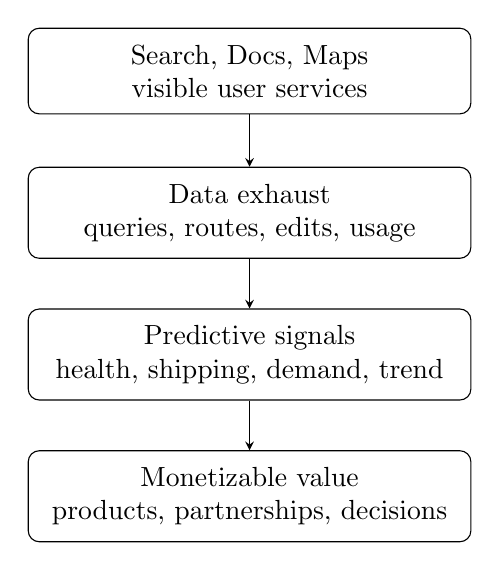
\begin{tikzpicture}[>=stealth]
\node[draw, rounded corners, align=center, text width=5.2cm, inner sep=6pt] (g1) at (0,0) {Search, Docs, Maps\\visible user services};
\node[draw, rounded corners, align=center, text width=5.2cm, inner sep=6pt] (g2) at (0,-1.8) {Data exhaust\\queries, routes, edits, usage};
\node[draw, rounded corners, align=center, text width=5.2cm, inner sep=6pt] (g3) at (0,-3.6) {Predictive signals\\health, shipping, demand, trend};
\node[draw, rounded corners, align=center, text width=5.2cm, inner sep=6pt] (g4) at (0,-5.4) {Monetizable value\\products, partnerships, decisions};
\draw[->] (g1) -- (g2);
\draw[->] (g2) -- (g3);
\draw[->] (g3) -- (g4);
\end{tikzpicture}
\caption{Transcript-derived reconstruction of how Google turns visible services into predictive value.}
\end{figure}

Kivel uses Google's size rhetorically rather than analytically:
\begin{equation}
\text{market cap} \approx \$2.4 \text{ trillion}.
\end{equation}
The force of the number is not in its exact financial interpretation. It is in the contrast with the humble origin point: a company that began by fixing search became one of the most consequential data-and-infrastructure firms in the world.

The health example clarifies the mechanism. Regional search spikes for symptoms become biomarkers, then data points, then public-health signals. Those signals can inform health organizations, clinicians, and even pharmaceutical or over-the-counter product planning. The company that began by indexing web pages now participates in the practical anticipation of disease patterns.

\subsection{Question \& Answer}

\paragraph{Question.} Why is trailing data nearly useless, and what replaces it?

\paragraph{Answer.} Because trailing data arrives after the strategic advantage has mostly evaporated. Quarterly reports tell us what happened. They do not tell us early enough what is about to happen. Kivel's substitute is the leading indicator: shipping activity, search behavior, satellite observation, lot inventory, and any other present signal that predicts future movement.

The lecture's asymmetry can be written as
\begin{equation}
\text{decision value}(\text{leading indicator})
>
\text{decision value}(\text{trailing report}).
\end{equation}
This is not a theorem but an operating principle. If official data tell us how many cars were sold last quarter, that information is already old. If current shipping patterns tell us that fewer cars are leaving port now, then a prediction about next quarter becomes actionable before the official report exists.

Kivel folds this back into a more general enterprise example. A logistics product may promise
\begin{equation}
\Delta \text{productivity} \approx 15\%.
\end{equation}
That number is not presented as a measured law. It is the sort of concrete business claim by which an offering becomes meaningful to a client. Yet even here the same warning returns: the first model may be simple, but the company must keep becoming more valuable, more relevant, and more sticky.

At this point the lecture pauses, briefly, for questions, and then turns. We have seen two major platform examples. Now Kivel narrows the field again and says, in effect: let us talk about industries.

\section{Industry-Specific Models: MedTech, Diagnostics, and Pharma}

The lecture's pivot back to industry specificity is crucial. Kivel explicitly says that pharmaceutical, diagnostic, and med-tech businesses are not interchangeable. Even inside life sciences, each sector carries a different business model.

Med tech becomes the sharpest example because it compresses technical success and commercial failure into the same space. A lab may achieve proof of concept. A device may work. A device may be safe. Yet the market question remains: who will adopt it, who will prescribe it, who will pay for it, and what service structure surrounds it?

The central tension can be written cleanly as
\begin{equation}
(\text{efficacious}\land \text{safe}) \not\Rightarrow \text{adopted}.
\end{equation}
This is the lecture's most important formal reconstruction. It captures exactly the obstacle Kivel is building toward. In med tech, technical success is necessary, but it is not sufficient.

The lecture's validated visual evidence belongs here.

\begin{figure}[htbp]
\centering

\includegraphics[width=0.92\linewidth]{lecture_03_figure_02.png}
\caption{MedTech framework slide with efficacy, validation, data, and remote-service dimensions.}
\end{figure}

The slide itself is not a workflow. It is a radial framework of simultaneous pressures:
\begin{equation}
\{\text{efficacy},\ \text{data-driven},\ \text{device validation},\ \text{remote service}\}.
\end{equation}

\begin{figure}[htbp]
\centering
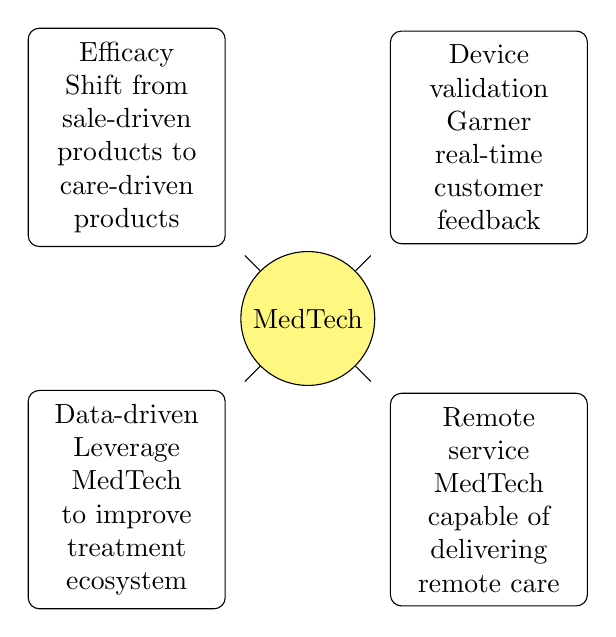
\begin{tikzpicture}
\node[draw, circle, minimum size=1.7cm, align=center, fill=yellow!50] (m) at (0,0) {MedTech};

\node[draw, rounded corners, align=center, text width=2.15cm, inner sep=5pt] (e) at (-2.3,2.3)
{Efficacy\\Shift from sale-driven\\products to\\care-driven products};

\node[draw, rounded corners, align=center, text width=2.15cm, inner sep=5pt] (v) at (2.3,2.3)
{Device validation\\Garner real-time\\customer feedback};

\node[draw, rounded corners, align=center, text width=2.15cm, inner sep=5pt] (d) at (-2.3,-2.3)
{Data-driven\\Leverage MedTech\\to improve\\treatment ecosystem};

\node[draw, rounded corners, align=center, text width=2.15cm, inner sep=5pt] (r) at (2.3,-2.3)
{Remote service\\MedTech capable of\\delivering\\remote care};

\draw (m) -- (-0.8,0.8);
\draw (m) -- (0.8,0.8);
\draw (m) -- (-0.8,-0.8);
\draw (m) -- (0.8,-0.8);
\end{tikzpicture}
\caption{Pocket-safe redraw of the MedTech framework visible in the lecture slide.}
\end{figure}

\subsection{Question \& Answer}

\paragraph{Question.} Why is ``safe and effective'' still not enough?

\paragraph{Answer.} Because the commercial system is not the same as the technical system. One must ask which clinicians adopt first, which specialists are influential, how fast the specialty changes its behavior, whether reimbursement exists, whether the product is direct-to-consumer or prescription-mediated, and whether the service structure supports remote or repeated use. Kivel's examples are pointed. Surgeons may be eager for new instruments; psychiatrists may be slower to adopt new technologies. A patient may see an advertisement, but if the doctor does not prescribe, the product does not sell.

That is the decisive lesson of the MedTech beat. In a simple consumer product the buyer and the user may be the same person. In med tech, the chain from innovation to payment is often multi-layered and institutionally constrained.

\subsection{Switching Costs, Segmentation, and the Late Examples}

Once this sector-specific pressure has been made vivid, the lecture widens again. The remaining examples may appear miscellaneous if we flatten them, but they are not miscellaneous. They are a final sweep of heuristics.

First comes switching cost:
\begin{equation}
\text{low switching cost for buyer}
\Rightarrow
\text{high churn risk for seller}.
\end{equation}
The lecture illustrates this with mobile carriers and gym memberships. Buyers like easy exit. Sellers dislike it because it creates turnover. Yet competitive pressure may force the seller to permit exactly that low-friction movement.

This is why Mint Mobile matters in the lecture. Mint uses T-Mobile's network, but reaches a different segment: bring your own device, no long contract, cheaper monthly access, less bandwidth privilege. The core idea is not merely telecom. It is segmentation. An incumbent model may work well and still miss an entire part of the market.

The same principle reappears in brand ladders. Toyota and Lexus, Nissan and Infiniti, Ralph Lauren and its internal hierarchy of labels: these examples all serve the same lesson. A firm can create adjacent brands or adjacent offers to reach people whom the original identity could not reach. The lecture's live exchange on exact automotive genealogy wanders somewhat, but the conceptual point remains sharp.

Digital commerce then supplies a new cluster of examples. Uber coordinates rides without owning cars. Airbnb coordinates lodging without owning rooms. Rent the Runway is not merely ``sharing'' but a personalized access model. The replenishment economy removes the need to remember to reorder household goods. The do-it-for-me service economy expands conveniences that once seemed reserved for the wealthy.

Travel becomes the last broad example before the close. What used to require a travel agent can now be built through search or generated through AI prompts. Here again Kivel's point is not that technology changes everything in the abstract. It is that changed technology permits new models of reaching the user.

The AI coda makes the same point one final time from the infrastructure side. A data center is a business. A data center in Norway, using a particular climate advantage, a particular energy profile, a particular funding structure, and a particular compute contract, begins to look like a business model. On the application side, tools such as Otter turn transcription into summary and summary into action items. The visible app is the surface; the model lies in where it sits in the value chain and what workflow it displaces.

The closing advice is therefore earned rather than generic. Do not overcomplicate the model. Understand the market dynamics. Be flexible. The companies that survive are the ones that see the future early enough to alter themselves.

\section{Summary}

This lecture begins with a handoff from customer discovery and ends with a warning about adaptability. Between those two points it builds a coherent sequence. First, a business model is the practical structure by which value is created, delivered, and captured. Second, channel design is not secondary to product design; the MolecularWare case makes that unmistakable. Third, successful companies survive by modifying their model before the old one collapses. Netflix does this across format, content, and access rules. Google does it by turning visible services into predictive signals. Med tech shows the sharpest tension of all: technical success does not guarantee adoption. The final lesson is therefore sober and operational. We should ask of any company not merely what it makes, but how it reaches the buyer, how it gets paid, and how it will change when its first successful arrangement is no longer enough.